\documentclass[11pt, a4paper]{article}

\usepackage{style}

\author{Vladislav Mlejnecký}

\title{%
  Číslicové zpracování signálů\\
  \large Úloha číslo 6.\\
  Přenosová funkce LTI, kmitočtová charakteristika, nástroje Matlab - II}

\begin{document}

    \maketitle

    \section{Zadání}
    
        \begin{enumerate}
            \item
            Ověřte vlastnosti filtrů IIR a FIR navržené pomocí funkcí Matlab, vyzkoušejte,co Matlab „vydrží“.
        \end{enumerate}
    
    \section{Výsledné grafy}
    
        \subsection{Filtr s aproximací butter}
            
            \begin{figure}[H]
                \centering
                \begin{minipage}{.5\textwidth}
                    \centering
                    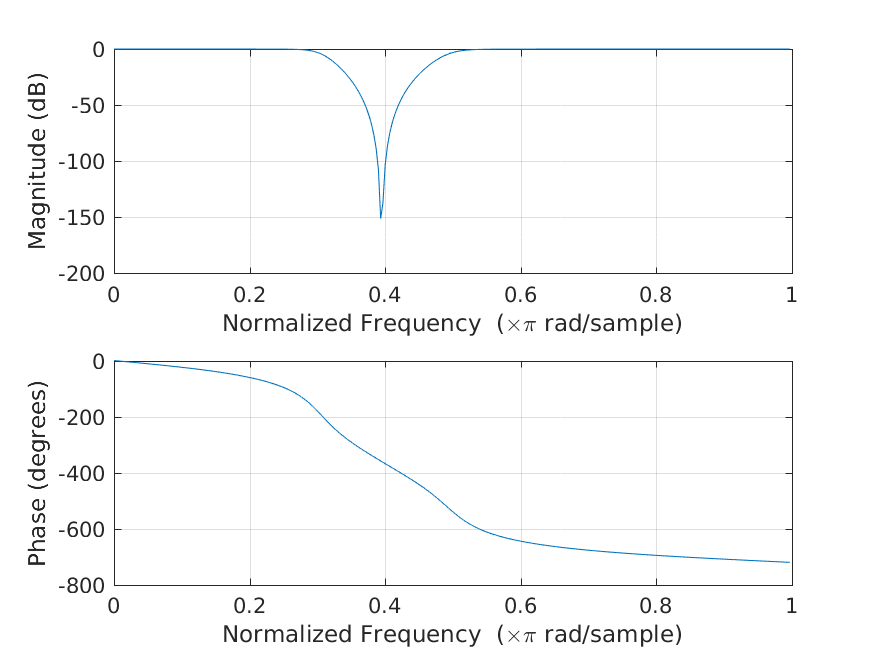
\includegraphics[width=.9\textwidth]{matlab/butter_n4.png}
                    \caption{Filtr 4. řádu s aproximací \textit{butter}}
                    \label{fig:1}
                \end{minipage}%
                \begin{minipage}{.5\textwidth}
                    \centering
                    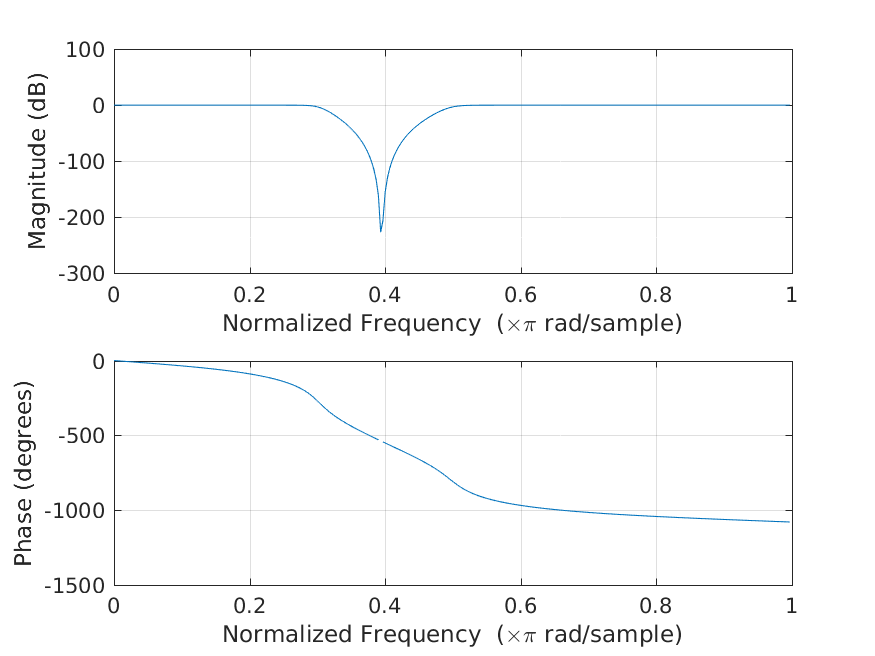
\includegraphics[width=.9\textwidth]{matlab/butter_n6.png}
                    \caption{Filtr 6. řádu s aproximací \textit{butter}}
                    \label{fig:2}
                \end{minipage}
            \end{figure}
        
            \begin{figure}[H]
                \centering
                \begin{minipage}{.5\textwidth}
                    \centering
                    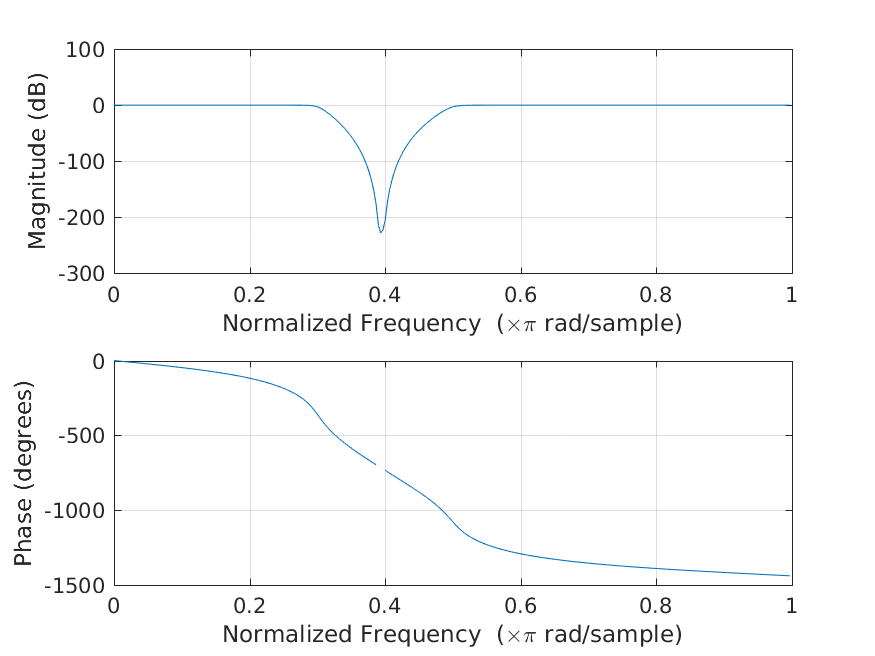
\includegraphics[width=.9\textwidth]{matlab/butter_n8.png}
                    \caption{Filtr 8. řádu s aproximací \textit{butter}}
                    \label{fig:3}
                \end{minipage}%
                \begin{minipage}{.5\textwidth}
                    \centering
                    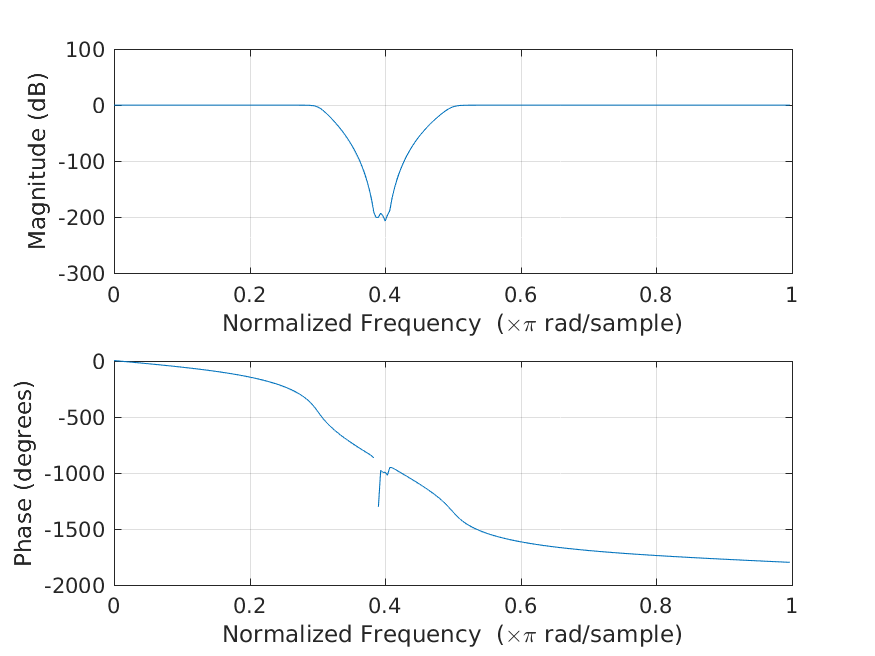
\includegraphics[width=.9\textwidth]{matlab/butter_n10.png}
                    \caption{Filtr 10. řádu s aproximací \textit{butter}}
                    \label{fig:4}
                \end{minipage}
            \end{figure}
            
        \subsection{Filtr s aproximací čebyšev 1. typu}
            
            \begin{figure}[H]
                \centering
                \begin{minipage}{.5\textwidth}
                    \centering
                    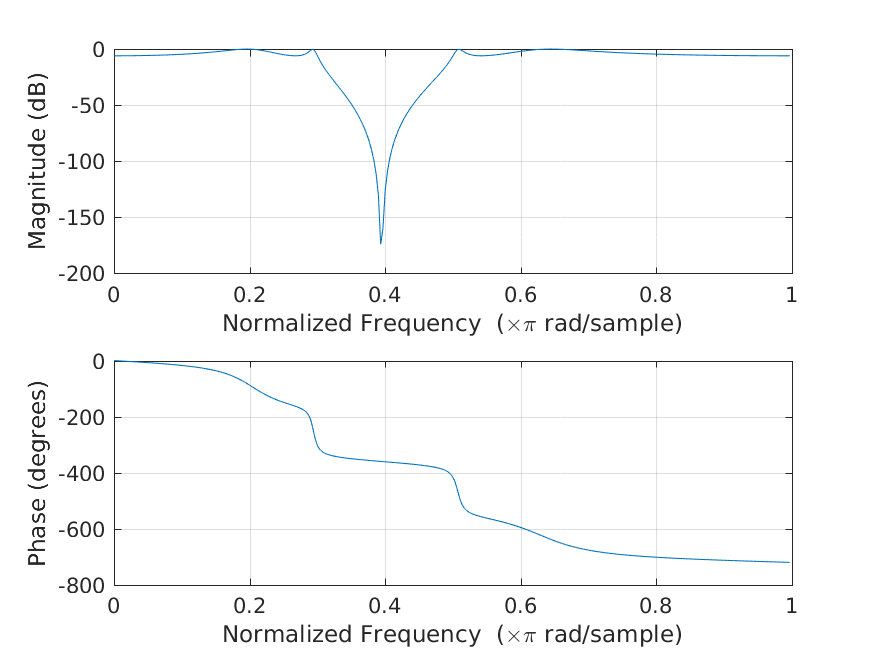
\includegraphics[width=.9\textwidth]{matlab/cheby1_n4.png}
                    \caption{Filtr 4. řádu s aproximací \textit{cheby 1}}
                    \label{fig:5}
                \end{minipage}%
                \begin{minipage}{.5\textwidth}
                    \centering
                    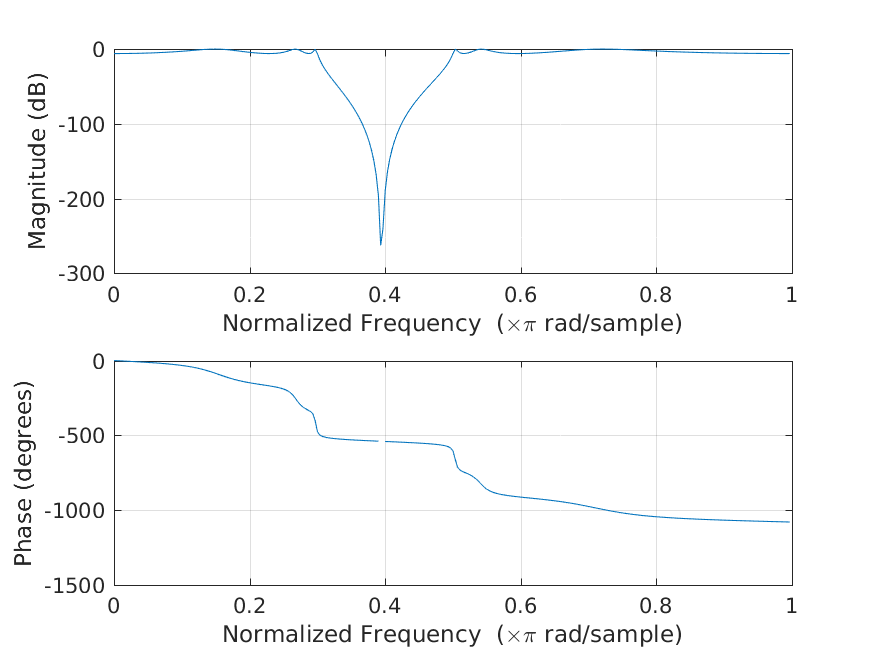
\includegraphics[width=.9\textwidth]{matlab/cheby1_n6.png}
                    \caption{Filtr 6. řádu s aproximací \textit{cheby 1}}
                    \label{fig:6}
                \end{minipage}
            \end{figure}
        
            \begin{figure}[H]
                \centering
                \begin{minipage}{.5\textwidth}
                    \centering
                    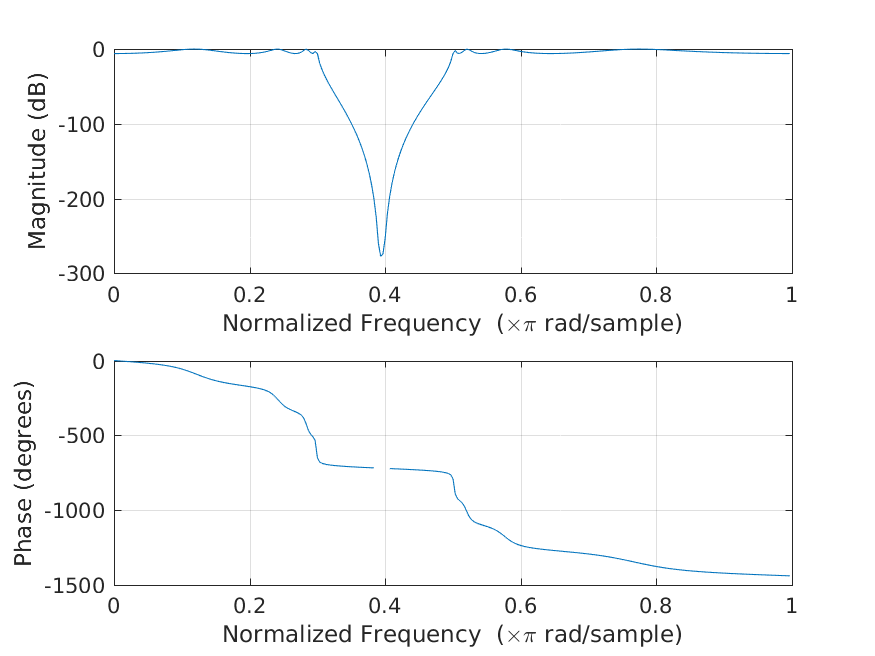
\includegraphics[width=.9\textwidth]{matlab/cheby1_n8.png}
                    \caption{Filtr 8. řádu s aproximací \textit{cheby 1}}
                    \label{fig:7}
                \end{minipage}%
                \begin{minipage}{.5\textwidth}
                    \centering
                    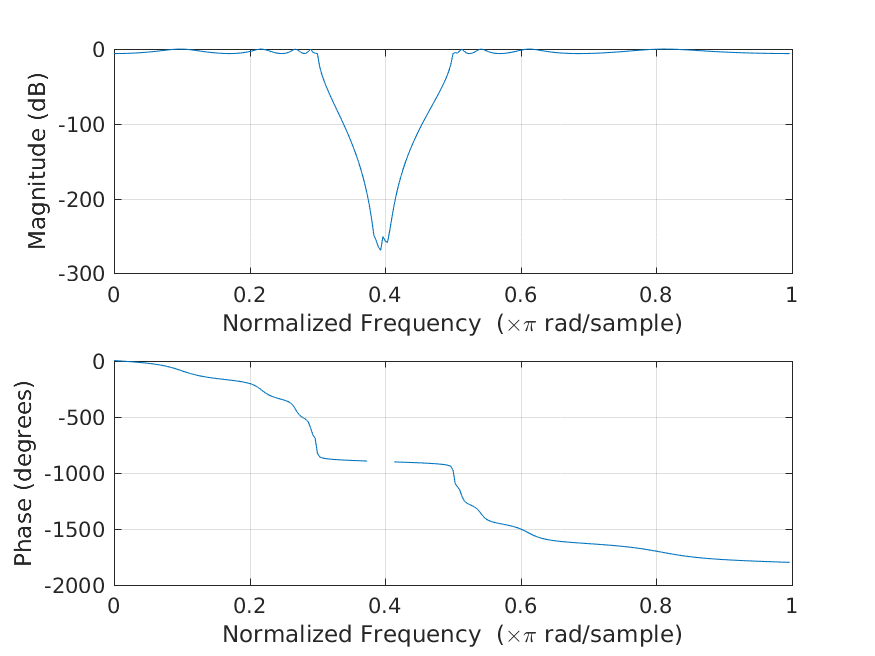
\includegraphics[width=.9\textwidth]{matlab/cheby1_n10.png}
                    \caption{Filtr 10. řádu s aproximací \textit{cheby 1}}
                    \label{fig:8}
                \end{minipage}
            \end{figure}
        
        \subsection{Filtr s aproximací čebyšev 2. typu}
            
            \begin{figure}[H]
                \centering
                \begin{minipage}{.5\textwidth}
                    \centering
                    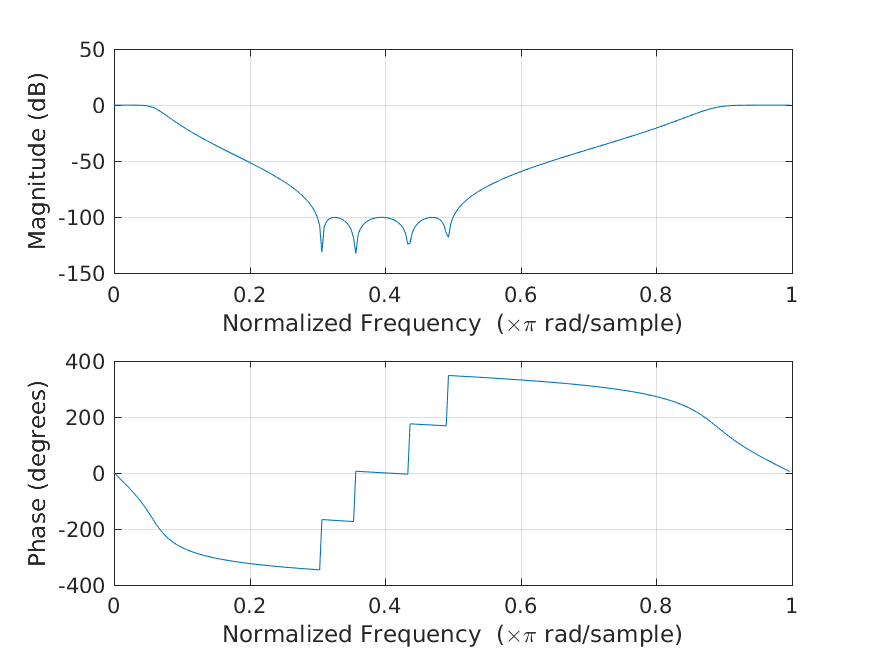
\includegraphics[width=.9\textwidth]{matlab/cheby2_n4.png}
                    \caption{Filtr 4. řádu s aproximací \textit{cheby 2}}
                    \label{fig:9}
                \end{minipage}%
                \begin{minipage}{.5\textwidth}
                    \centering
                    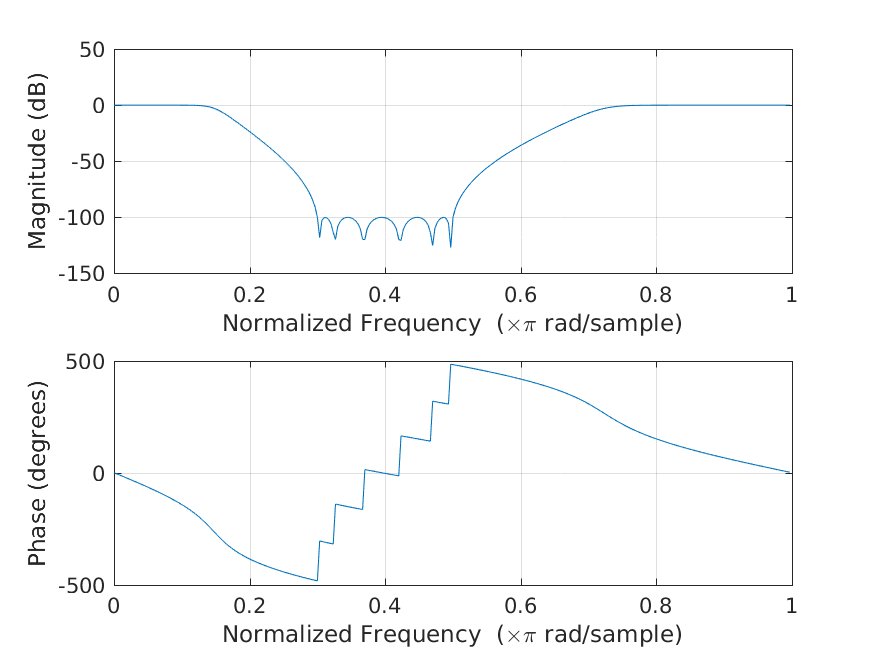
\includegraphics[width=.9\textwidth]{matlab/cheby2_n6.png}
                    \caption{Filtr 6. řádu s aproximací \textit{cheby 2}}
                    \label{fig:10}
                \end{minipage}
            \end{figure}
        
            \begin{figure}[H]
                \centering
                \begin{minipage}{.5\textwidth}
                    \centering
                    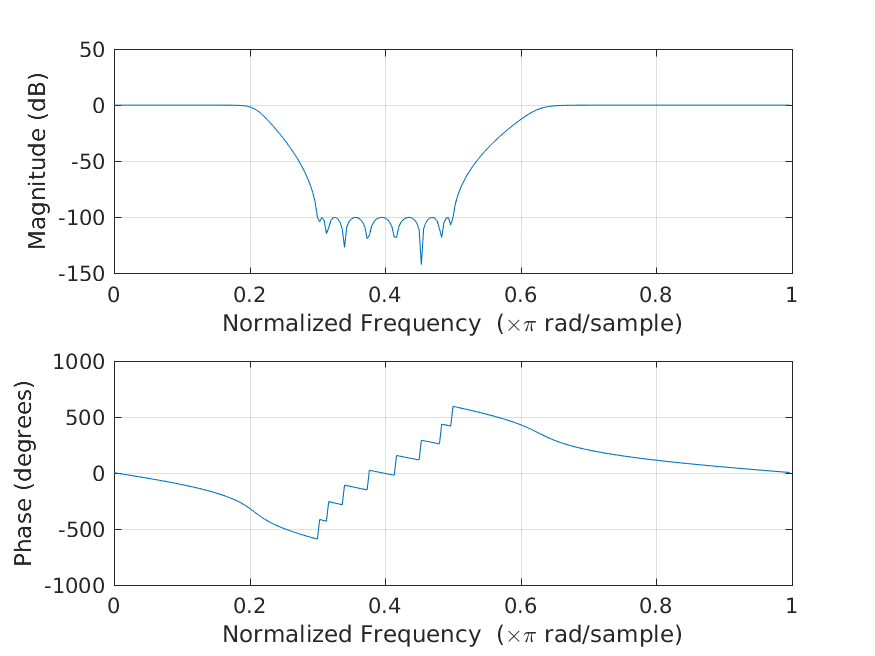
\includegraphics[width=.9\textwidth]{matlab/cheby2_n8.png}
                    \caption{Filtr 8. řádu s aproximací \textit{cheby 2}}
                    \label{fig:11}
                \end{minipage}%
                \begin{minipage}{.5\textwidth}
                    \centering
                    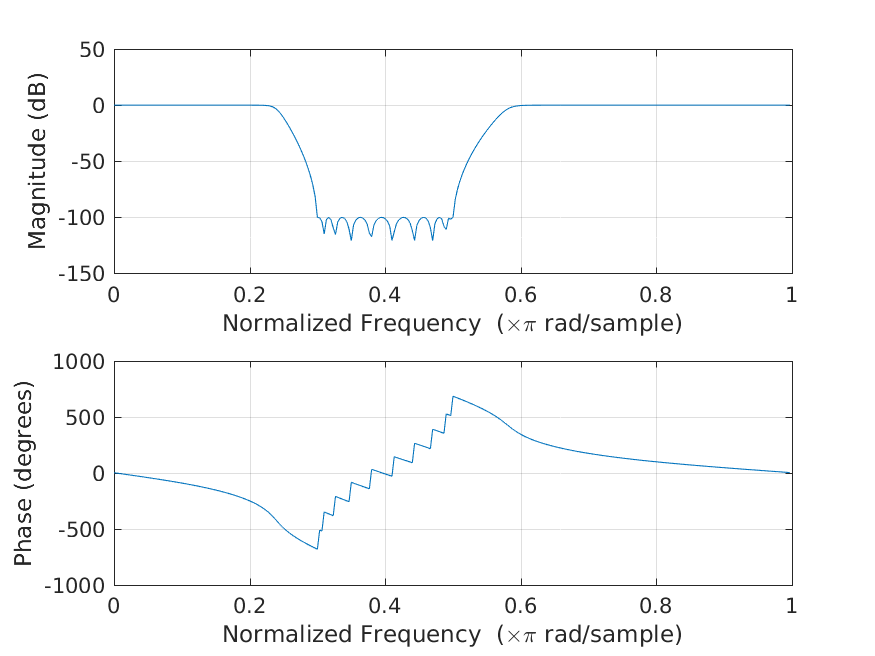
\includegraphics[width=.9\textwidth]{matlab/cheby2_n10.png}
                    \caption{Filtr 10. řádu s aproximací \textit{cheby 2}}
                    \label{fig:12}
                \end{minipage}
            \end{figure}
        
        \subsection{Filtr s eliptickou aproximací}
            
            \begin{figure}[H]
                \centering
                \begin{minipage}{.5\textwidth}
                    \centering
                    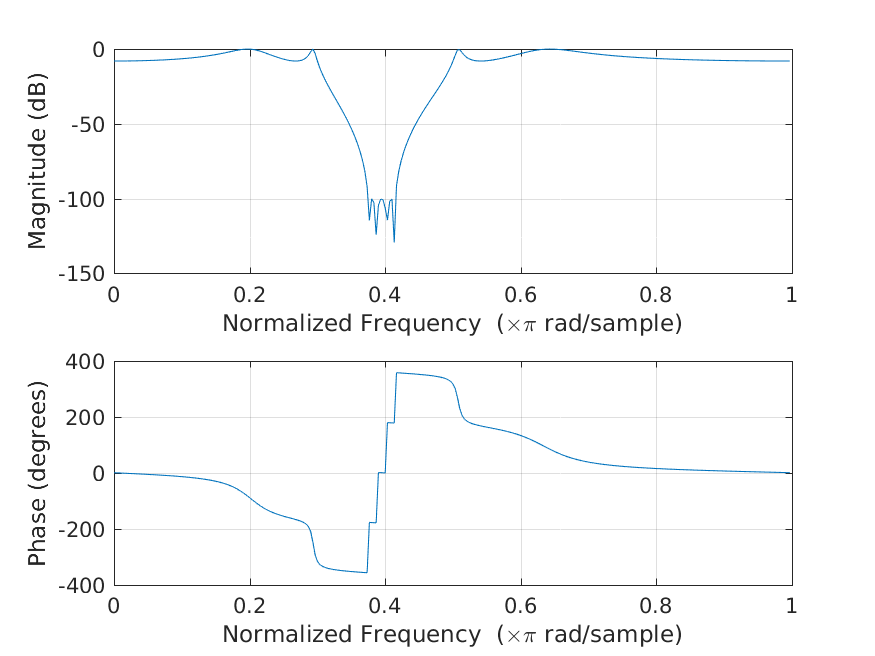
\includegraphics[width=.9\textwidth]{matlab/ellip_n4.png}
                    \caption{Filtr 4. řádu s aproximací \textit{ellip}}
                    \label{fig:13}
                \end{minipage}%
                \begin{minipage}{.5\textwidth}
                    \centering
                    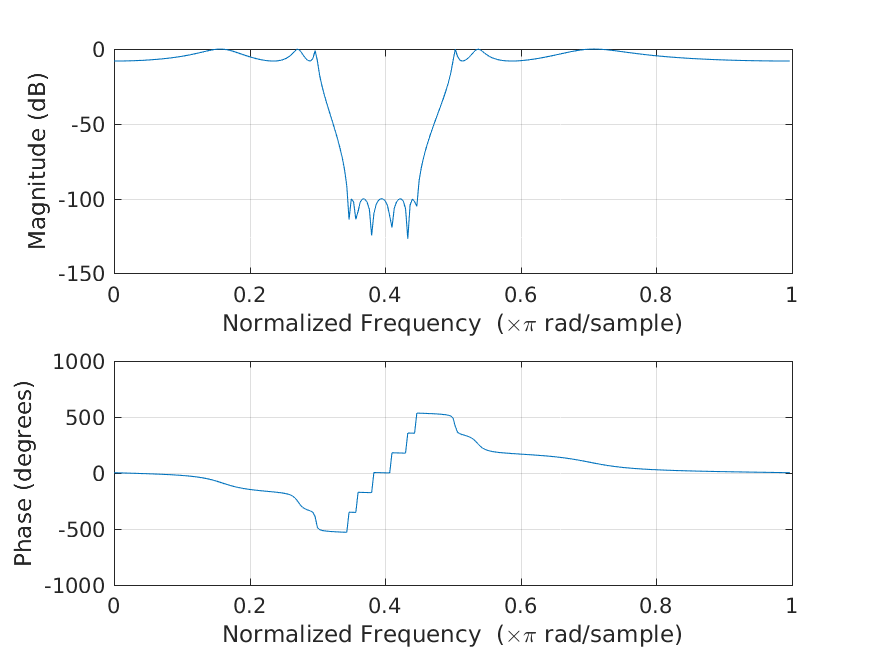
\includegraphics[width=.9\textwidth]{matlab/ellip_n6.png}
                    \caption{Filtr 6. řádu s aproximací \textit{ellip}}
                    \label{fig:14}
                \end{minipage}
            \end{figure}
        
            \begin{figure}[H]
                \centering
                \begin{minipage}{.5\textwidth}
                    \centering
                    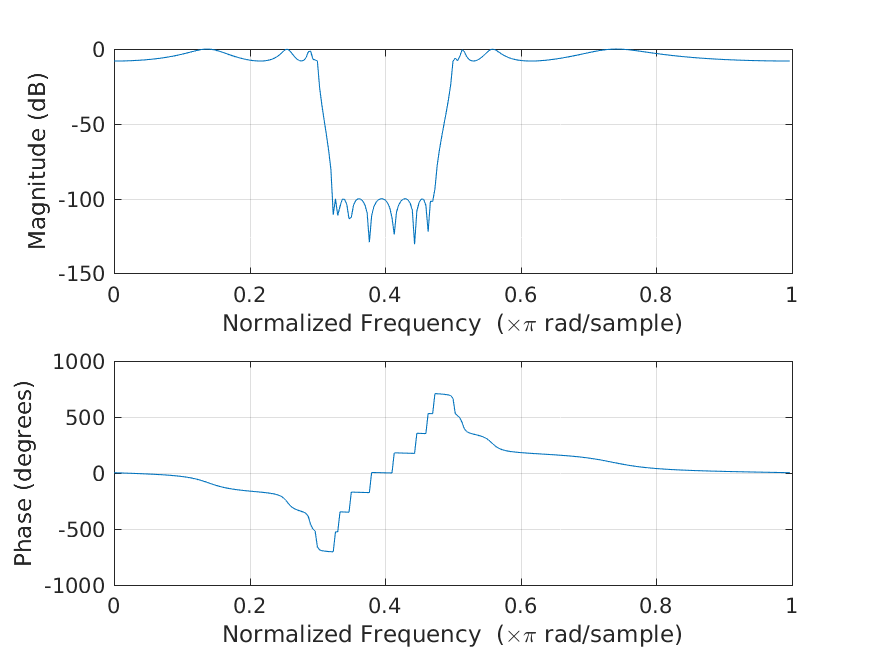
\includegraphics[width=.9\textwidth]{matlab/ellip_n8.png}
                    \caption{Filtr 8. řádu s aproximací \textit{ellip}}
                    \label{fig:15}
                \end{minipage}%
                \begin{minipage}{.5\textwidth}
                    \centering
                    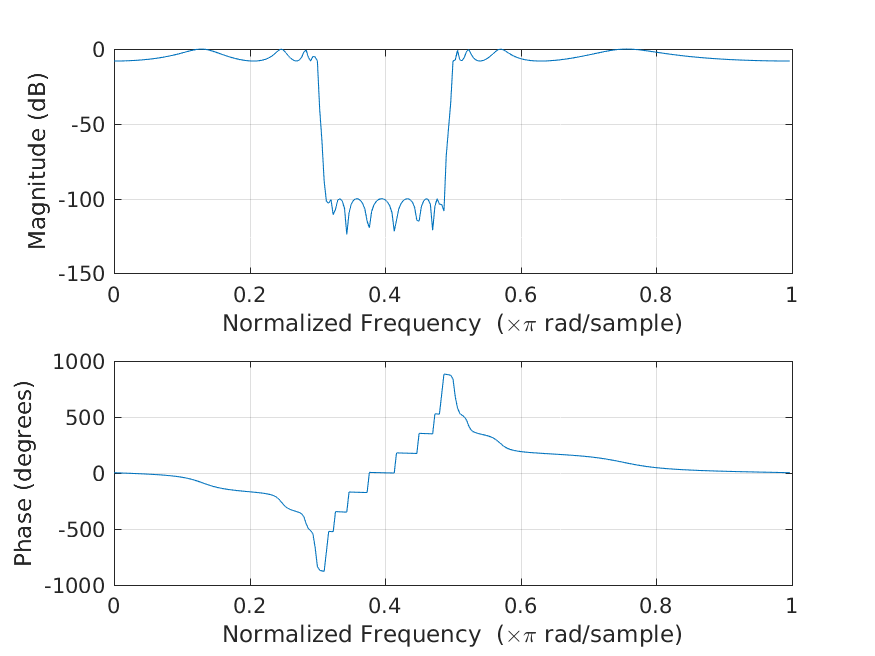
\includegraphics[width=.9\textwidth]{matlab/ellip_n10.png}
                    \caption{Filtr 10. řádu s aproximací \textit{ellip}}
                    \label{fig:16}
                \end{minipage}
            \end{figure}
            
    \section{Výpis zdrojového kódu}
    
\begin{lstlisting}[language=matlab, frame=single]    
%butter aproximation
for n = 4:2:10
    Wp=[0.3 0.5];
    [b,a] = butter(n, Wp, 'stop'); 
    
    h = figure();
    freqz(b, a, 300);
    
    saveas(h, ['butter_n' int2str(n) '.png']);
    close(h);
    clear h;
end

%cheby 1 aproximation
for n = 4:2:10
    Wp = [0.3 0.5];
    Rp = 6;

    [b,a] = cheby1(n, Rp, Wp, 'stop');
    
    h = figure();
    freqz(b, a, 300);
    
    saveas(h, ['cheby1_n' int2str(n) '.png']);
    close(h);
    clear h;
end

%cheby 2 aproximation
for n = 4:2:10
    Wp = [0.3 0.5];
    Rs = 100;

    [b,a] = cheby2(n, 100, Wp, 'stop');
    
    h = figure();
    freqz(b, a, 300);
    
    saveas(h, ['cheby2_n' int2str(n) '.png']);
    close(h);
    clear h;
end

%elliptic aproximation
for n = 4:2:10
    Wp = [0.3 0.5];
    Rs=100;
    Rp=8;
    
    [b,a] = ellip(n, Rp, Rs, Wp, 'stop');
    
    h = figure();
    freqz(b, a, 300);
    
    saveas(h, ['ellip_n' int2str(n) '.png']);
    close(h);
    clear h;
end
\end{lstlisting}

\end{document}
